\documentclass[a4paper,10pt]{article}
% Use ctrl + alt + V to view live pdf

% Packages
\usepackage[utf8]{inputenc} % For encoding
\usepackage[T1]{fontenc} % Better handling of accented characters and hyphenation
\usepackage{microtype} % Improves spacing and justification
\usepackage{amsmath, amssymb} % For equations and symbols
\usepackage{graphicx} % For including graphics/images
\usepackage{caption} % For customizing figure and table captions
\usepackage{subcaption} % For subfigures and subcaptions
\usepackage{float} % For fixing figure and table positions
\usepackage{booktabs} % For professional-looking tables
\usepackage{siunitx} % For consistent typesetting of units and numbers
\usepackage[margin=2cm]{geometry} % Adjusts page margins
\usepackage{fancyhdr} % For custom headers and footers
\usepackage{lmodern} % For a professional-looking font (main body font)
\usepackage{titlesec} % For title customization
\usepackage{array} % For custom table formatting
\usepackage[colorlinks=true, linkcolor=black, citecolor=blue, urlcolor=blue]{hyperref} % Colored links without boxes
\usepackage{cleveref} % For improved cross-referencing    
\usepackage{multirow}
\usepackage{enumitem}
\usepackage{listings}
\usepackage{xcolor}
\usepackage{textcomp}
\usepackage{tabularx}
\usepackage{changepage}
\usepackage{tikz}
\usepackage{pdfpages}
\usetikzlibrary{shapes.geometric, arrows}
\newcolumntype{Y}{>{\centering\arraybackslash}X}
% Reduce spacing before and after \section
% \titlespacing{\section}{0pt}{1.0em}{0.5em}
% Reduce spacing before and after \subsection
% \titlespacing{\subsection}{0pt}{0.8em}{0.3em}


\lstdefinestyle{verilog-style}{
    language=Verilog,
    basicstyle=\ttfamily\footnotesize,
    keywordstyle=\bfseries\color{blue},
    commentstyle=\itshape\color{gray},
    stringstyle=\color{red},
    numbers=left,
    numberstyle=\tiny\color{gray},
    stepnumber=1,
    breaklines=true,
    showstringspaces=false,
    frame=single
}
\lstset{style=verilog-style}
\lstset{captionpos=b}
\lstset{basicstyle=\ttfamily\scriptsize} 
\renewcommand{\lstlistingname}{Program}

% Custom settings
\pagestyle{fancy}
\fancyhf{}
\fancyhead[L]{\textit{GB3 - Risc-V Processor}} % Header left
\fancyhead[R]{\textit{Will Hewes - wh365}} % Header right 
\fancyfoot[C]{\thepage} % Footer center
\setlength{\headheight}{15pt} % Header height
\setlength{\parindent}{0em} % Indentation for paragraphs
\setlength{\parskip}{0.2em} % Add spacing between paragraphs
\setlength{\abovedisplayskip}{0.5em}
\setlength{\belowdisplayskip}{0.5em}
\setlength{\abovedisplayshortskip}{0.5em}
\setlength{\belowdisplayshortskip}{0.5em}
\setlist{topsep=0em, partopsep=0em, itemsep=0em, parsep=0em}

\graphicspath{{Images/}}

% \renewcommand{\arraystretch}{1.2}

% Title formatting
\renewcommand{\maketitle}{
    \begin{center}
        \LARGE \textbf{ENGINEERING TRIPOS PART IIA} \\ 
        \vspace{0.5em}
        \Large \textbf{GB3 - Risc-V Processor} \\ 
        \vspace{0.5em}
        \textbf{Final Report} \\
        \large Group 4 - Resource Usage \\
        \vspace{1em}
        \large Will Hewes - wh365 \\ 
        Pembroke College \\ 
        \vspace{0.5em}
    \end{center}
}

\begin{document}
\pagenumbering{gobble}
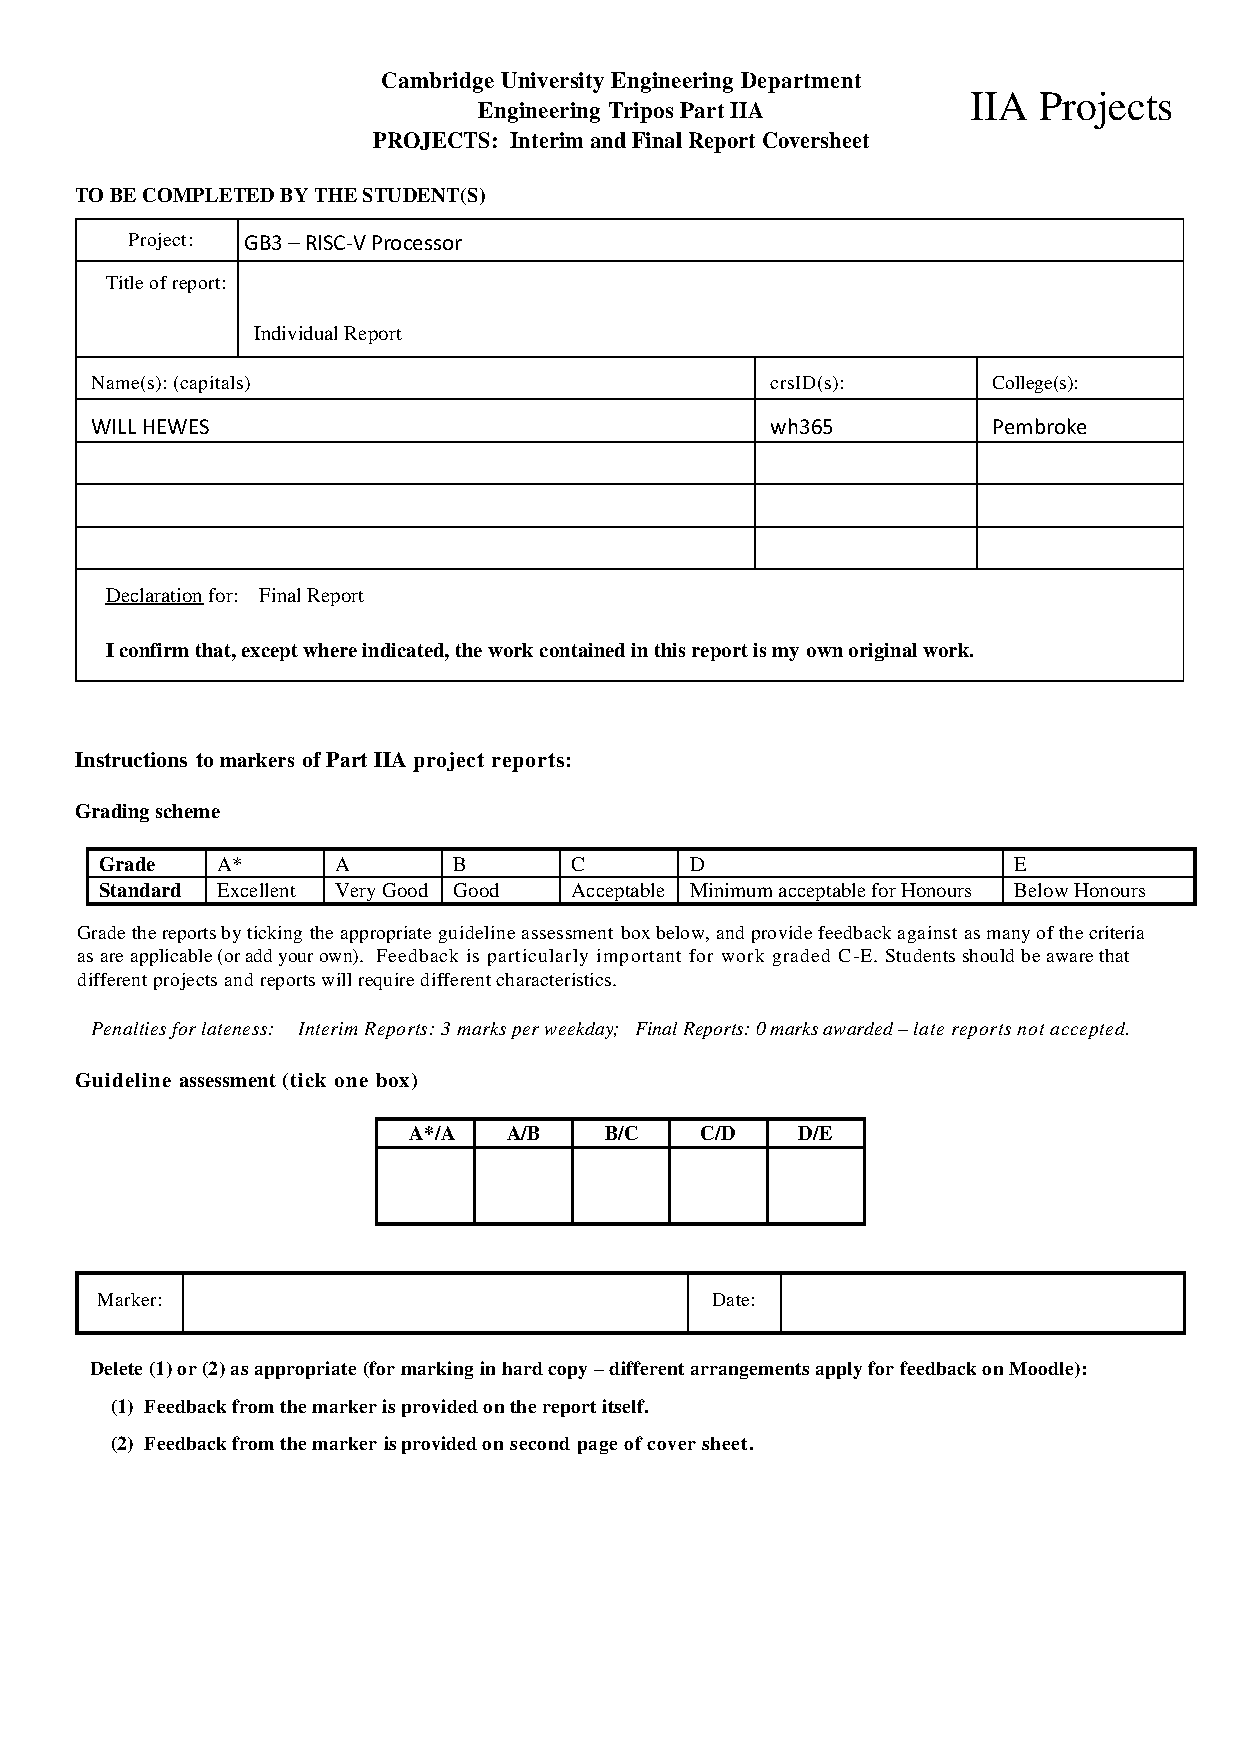
\includepdf[pages=-]{Handouts/IIA Project Coversheet Feedback Final Report.pdf}
\maketitle
\hrule
\tableofcontents
\newpage
\pagenumbering{arabic} \setcounter{page}{1}
% No more than 8 A4 sides, excluding appendices
% Include tables and descriptions in resource usage?

\section{Introduction}
\label{sec:Introduction}
% This section should give a detailed introduction to the changes
% you have implemented for your role on the team 
% (1 A4 side)

This project involves the collaborative design and implementation 
of a RISC-V processor on an iCE40 FPGA device. 
The overarching aim is to optimise 
the processor design with respect to its 
performance, power dissipation, and resource usage, 
while balancing trade-offs between these three aspects. 
Each team member is responsible for focusing on one of the three aspects
and my reports focus on the resource usage of the design.
This report is the final report for this project.

In the first report we evaluated three programs as a baseline against
which our improvements could be compared.
The first of these three porgrams was \texttt{hardwareblink},
a program which relied purely on combinational and sequential logic
to blink an LED on the FPGA,
bypassing the processor core entirely. 
As a result it had very low resource utilisation across the board.
The second program evaluated was \texttt{softwareblink},
which performed the same task but instead implemented through software,
utilising the sail-core processor.
As a result, the design used a much larger number of logic cells,
and also introduced the usage of a few other primitive cells such as 
block RAMs and DSP blocks.
The final program was \texttt{bubblesort}, which would perform a 
bubblesort algorithm and blink the LED to confirm it was finished.
Due to the increased complexity of the program,
the logic cell utilisation was greater than for \texttt{softwareblink},
but crucially the other primitives did not increase, 
as they relied primarily on their design within the verilog files.
The final test would be to process 
a new, unseen program under our implementation and evaluate it for its 
resource usage, performance and power dissipation.
As such we chose to base our testing primarily 
on the more complex \texttt{bubblesort},
allowing us to push the processor further,
offering a more representative view of our design.
It should be noted the other programs were still tested
to ensure functionality and check progress,
they were just less emblematic of our implementaions capabilities.

The baseline implementation on the FPGA showed several inefficiencies 
in its core design and made poor use of 
some of the resources available on the board. 
Before describing the changes made, it's helpful to briefly explain 
what those resources are and how they affect the processor.

Logic cells, or LCs, are the basic building blocks used to 
implement logic on the FPGA. 
They include components like look-up tables and flip-flops, 
and are used for almost everything, including 
arithmetic, control signals, and registers. 
Because almost everything in the design depends on logic cells in some way, 
reducing how many are used was the main goal throughout the project.
The changes that directly improved LC usage primarily came from
cleaning up registers, wires, and other redundant logic where possible.
One noteable example of this was reducing a multiplexing wire signal
from 32 bits down to 11 bits. These examples will be discussed in more detail
in the body of the report.

Other primitives available on the board are similarly powerful,
though they have a key difference - they are fixed for a given implementation
on the microprocessor.
This means that whereas LCs will increase and potentially become limiting
for a particularly complex program, 
other primitives such as block RAMs, DSP registers, and buffers
will not increase outside of the capacity of the board if designed properly.

Block RAMs are small dedicated memory blocks built into the FPGA. 
They're useful when a design needs to store more data 
than would be practical with flip-flops alone. 
In the baseline implementation, 
they were used by certain parts of the processor 
such as the register file and CSR logic. 
By removing CSR logic from the design,
the number of block RAMs used was reduced 
from 20 to 12 of the 30 available,
meaning that more memory functions could be moved to the RAM 
in order to preserve logic cells.
Unfortunately these changes could not be implemented due to time constraints,
but the plan was to ...

DSP blocks are specialised units designed for fast arithmetic. 
Instead of building adders and multipliers out of regular logic, 
the FPGA provides a few dedicated DSP blocks that are faster and use less space. 
The baseline design didn't use any of these, 
relying entirely on logic cells even for basic addition. 
One of the most significant alterations to the base implementation
was forcing the \textit{adder.v} to make use of these DSP blocks
for addition and subtraction, 
freeing up LUTs to be used in more sophisticated logic.
Implementing this change reduced the LC usage by ..., 
at the expense of 3 of the 8 DSP blocks available,
leaving room for further improvement in this regard.

In addition to these changes that were successfully implemented,
there are many that ...

\newpage

\section{Design Strategy}
\label{sec:Design_Strategy}
% Describing the specific design strategy employed for your role in the team (0.5-1 A4 side)
% Timeline diagram?
% Include subsection on the baseline processor, both description of its structure and resource usage

As I was initially unfamiliar with processor and FPGA design at this level, 
the early stages of the project were spent working through the course material 
and exploring online resources to build a clearer understanding of 
where changes could be most effectively targeted. 
This initial research was followed by a series of small, 
hands-on changes to the Verilog code, 
helping build familiarity with the processor's structure and behaviour.
In hindsight, these early edits were made 
without a broader design strategy in place, 
but they laid the groundwork for a more focused and informed optimisation approach 
that developed as the project progressed.
This unstructured approach naturally led to a few early mistakes, 
such as unintentionally breaking functionality or introducing hard-to-trace bugs.
These mistakes will be discussed more in Section \ref{sec:Problems_Encountered}.
These issues highlighted the need for a more disciplined workflow, 
which later included stricter version control, 
more careful integration with other modules, 
and simulations to verify that signals behaved as expected after changes.

As a team we worked together through git, allowing us to collaborate effectively.
We set up different branches from the \texttt{main} for each of us to use, 
with the plan being that we would work on some changes independently 
and then merge our changes cohesively.

A significant part of the optimisation process involved 
carefully examining the Verilog source files to understand 
the structure and interaction of each component
across multiple files. 
This required tracing signal flow through the datapath and control logic, 
identifying where logic or memory resources were being used inefficiently, 
and confirming whether particular subsystems - 
such as CSRs or multiplexer paths - 
were functionally active during execution. 
Pattern-matching tools like \texttt{grep} were used extensively 
to locate signal definitions and check bit widths, 
while simple simulation testbenches were created to verify specific behaviours,
most notably during the beleaguered formulation of the DSP blocks.
These methods helped build a reliable picture of the design's internal behaviour 
and revealed opportunities to safely eliminate or simplify hardware blocks 
without compromising core functionality.

After using these methods to identify and eliminate innefficiencies within the code,
these changes would be uploaded to git for integration with the other branches,
allowing us to work independently on our seperate focus and
providing an easy way to handle merge conflicts.

Unfortunately, this is another aspect where planning would have made a significant
improvement to our working procedure. 
As there was only one FPGA, our individual changes would be applied and
though they would successfully synthesise and be routed,
often the functionality would be broken and we would be unable to tell until 
the code could be tested on the FPGA when we would all meet again.
This meant that much of our time was spent working on changes that would 
need to be extensively debugged, and unfortunately many of these initial changes
would in the end remain unimplemented due to time constraints.

\section{Design Description}
\label{sec:Design_Description}
% For the components you implemented for your team (regardless of your role) (2-3 A4 sides)
% Include diagram on DSP blocks?
% Mention how your changes affect the other aspects
% Summarise original behaviour, describe original behaviour, justify it

The changes made during this project were, for the most part, 
minor and locally scoped optimisations rather than sweeping architectural overhauls. 
The aim throughout was to reduce resource usage on the FPGA - 
specifically the logic cell count  - 
without compromising the functional correctness of the processor. 
While logic cells were the primary focus, 
some changes also impacted the usage of other board primitives 
such as block RAMs and DSP blocks. 

Each optimisation was applied as discussed in earlier sections,
incrementally and tracked using Git, 
with synthesis reports logged at every stage to assess their effect. 
The following subsections outline each of these changes, 
along with their motivation, implementation, and observed impact. 
Where relevant, small pieces of code are shown in the main body of the report, 
while longer or supporting code is included in the appendix.

\subsection{Clock Gating}
\label{sec:Gating}

One of the earliest changes involved modifying the program counter (PC) logic 
to reduce unnecessary switching activity during pipeline stalls. 
In the baseline implementation, the PC would increment 
on every clock cycle regardless of whether the pipeline was stalled, 
resulting in wasted transitions and toggling of downstream logic even 
when no useful computation was occurring.

To address this, support for gated updates to the program counter was introduced. 
This involved modifying the \texttt{program\_counter.v} module to accept 
a new \texttt{write\_enable} signal, 
allowing updates to be conditionally applied only when 
pipeline progression was required. 
The \texttt{cpu.v} module was updated to assert this signal whenever 
the \texttt{stall} flag was low, 
ensuring that the PC would remain stable during pipeline stalls. 
The signal was then routed through \texttt{top.v} to maintain module connectivity.

This change primarily aimed to reduce dynamic power dissipation by 
avoiding unnecessary switching in the PC logic. 
While the overall resource saving was modest - 
freeing approximately 9 logic cells - 
it represents an important step in selectively controlling register updates. 
It also clarified the flow of stall logic through the processor 
and established a cleaner separation between control and datapath behaviour. 

One trade-off, however, was a slight increase in global buffer (GB) usage, 
rising from 5 to 6 out of the 8 available on the iCE40 device. 
Global buffers are specialised routing resources used to 
distribute high-fanout signals - 
such as clocks or enables - efficiently across the FPGA fabric. 
Their usage ensures consistent signal timing over long distances, 
especially when a control signal must drive registers in multiple modules. 
The increase was likely due to the new 
\texttt{pc\_write\_enable} signal being propagated through 
several layers of control and datapath logic, 
requiring global routing resources to maintain timing closure.
This is not a key resource in the same way that LUTs and flip-flops are, 
and so a minor increase in GB usage is not considered critical. 
Provided the design remains within the hardware limit of 8, 
such changes are acceptable if they simplify control signalling or improve timing.

The impact of this modification is 
summarised in Table \ref{tab:Program_Counter} in the Appendix.

\subsection{Signal Width Reduction}
\label{sec:Signal_Width}

Another optimisation involved reducing the width of a control signal used in 
the execution-to-memory pipeline stage. 
This signal, \texttt{ex\_cont\_mux\_out}, 
is used to carry control values from the decode 
stage into the execution stage, 
particularly for managing behaviours such as branching, memory operations, and ALU control. 
In the baseline implementation, this signal was declared as 32 bits wide, 
despite the fact that only the lower 11 bits 
were ever referenced or extracted in downstream modules. 
This resulted in an oversized bus that incurred extra logic and routing 
costs without delivering any functional benefit.

To identify the mismatch, \texttt{grep} was used to trace the usage of 
\texttt{cont\_mux\_out} throughout the Verilog files. 
This revealed that only specific slices of the signal were ever used, 
confirming that the top 21 bits could be safely discarded. 
With this knowledge, a dedicated 11-bit multiplexer module, 
\texttt{mux2to1\_11bit}, was written and substituted alongside the 
generic 32-bit \texttt{mux2to1}. 
The change required updating the 
module instantiation and associated wiring, 
but left the logic semantics unchanged.
This initial segment of code is shown in Program \ref{prog:mux_11bit}
in the Appendix for completeness.

After implementing this successful change, 
reducing logic cell usage but maintaining functionality of the program,
this was expanded upon to make this approach more flexible and maintainable.
The \texttt{mux2to1} assignment was expanded to support a parameterised width, 
allowing the same module to be reused in other parts of the design 
without hardcoding the bit width. 
This is shown in Program \ref{prog:mux} below. \cite{FPGA_optimization}

\begin{lstlisting}[style=verilog-style, caption=
    {Generic width multiplexer}, label={prog:mux}]
module mux2to1_param #(parameter WIDTH = 32)
( // Example instantiation: mux2to1_param #(.WIDTH(32))
    input  [WIDTH-1:0] input0,
    input  [WIDTH-1:0] input1,
    input              select,
    output [WIDTH-1:0] out
);
    assign out = (select) ? input1 : input0;
endmodule
\end{lstlisting}

This improvement reduced logic cell usage by 25 LUTs, as shown in 
Table \ref{tab:Mux} in the Appendix.

It should be noted that some widths were kept at 32 bits,
despite possessing redundancy in their width.
These were left unchanged as, 
although reducing their width would result in slightly fewer LUTs being used,
leaving their widths at 32 bits with the generic parameter multiplexing 
ended up reducing the delay from around 76ns to 69ns,
producing an unnaccounted for reduction in delay of 10\%.
In the future, this consequence would have to be probed further
to determine the root cause, but due to time constraints this was not possible.
There may be a more optimal configuration that could reduce resource usage
and improve timing further, but this was not worked out.

\subsection{DSP Substitution}
\label{sec:DSP}

Another important optimisation involved offloading arithmetic logic 
from general-purpose logic cells to dedicated DSP blocks on the FPGA. 
In the baseline implementation, the adder logic used for core operations 
such as basic arithmetic and branch comparisons was fully implemented in LUT-based logic, 
consuming a significant number of logic cells and contributing to routing congestion. 

To address this, the adder was restructured around 
the iCE40-specific \texttt{SB\_MAC16} primitive, 
which provides integrated adder functionality
along with a few other unused functions. 

In order to shift arithmetic operations over to the DSP,
the \texttt{SB\_MAC16} has to be explicitly declared,
otherwise the synthesis tools will just use general purpose LUTs instead.
This was implemented in the \texttt{adder.v} module, 
where the 32-bit operands were split into upper and lower 16-bit segments 
and mapped to the DSP's internal A, B, C, and D inputs. 
Parameterisation via \texttt{defparam} was used to configure the carry chain 
and data routing between the top and bottom halves of the DSP.
This is displayed in Program \ref{prog:DSP} in the Appendix.

This module was then instantiated within the ALU, allowing RISC-V instructions 
that required add or subtract operations to route through the DSP instead 
of a traditional behavioural adder. 
In order to implement addition, initially a wire was created that could
hold the 2s complement of a wire, as shown below in Program \ref{prog:2s_complement}.

\begin{lstlisting}[style=verilog-style, caption=
    {2s compliment}, label={prog:2s_complement}]
wire [31:0] B_neg = ~B + 1;
\end{lstlisting}

However, this unnecessarily increased complexity, and so instead
The control signal \texttt{is\_sub} was added to dynamically toggle between 
addition and subtraction by setting the 
\texttt{ADDSUBTOP} and \texttt{ADDSUBBOT} inputs. 

This is then instantiated in module \texttt{alu.v}
as shown below in Program \ref{prog:alu} below.

\begin{lstlisting}[style=verilog-style, caption=
    {is\_sub implementation within alu.v}, label={prog:alu}]
/*
 *	ADD
 */
`kSAIL_MICROARCHITECTURE_ALUCTL_3to0_ADD:	begin
	do_sub = 1'b0;
	ALUOut = add_result;
end
/*
 *	SUBTRACT
 */
`kSAIL_MICROARCHITECTURE_ALUCTL_3to0_SUB:	begin
	do_sub = 1'b1;
	ALUOut = add_result;
end
\end{lstlisting}

Following this change, logic cell usage was reduced by 94 LUTs, 
at the cost of 3 out of 8 available DSP blocks. 
As mentioned in Section \ref{sec:Introduction},
this increase in the usage of DSPs is not a negative,
as they are fixed hardware components with few other uses.
Shifting the simple arithmetic operations from 
far more malleable LUT and flip-flops over to the specialised DSPs
not only expands the capacity for software complexity on the board
but also improves the performance,
as DSPs are optimised for fast arithmetic calculations.

A simplified diagram illustrating the data path through the DSP adder 
is provided in Figure~\ref{fig:dspblock} in the Appendix.

\subsection{CSR}
\label{sec:CSR}

The most impactful change made to the processor was the complete removal of the 
Control and Status Register (CSR) logic. 
CSRs are a core but optional component of the RISC-V architecture specification, 
primarily used to support privileged operations such as 
trap handling, performance counters, environment configuration, and interrupt control. 
In a full system, CSR instructions are essential for switching between user and machine 
modes, managing exceptions, and interacting with the operating system. \cite{CSR}

However, for the purposes of this project, none of the benchmark programs utilised 
any CSR-related functionality. 
The processor ran entirely in \textit{machine mode}, 
the highest privilege level defined in the RISC-V specification. 
In this simplified configuration, 
there was no support for exception handling, privilege escalation, 
or multiple execution contexts. 
As a result, the Control and Status Register (CSR) subsystem - 
which is primarily intended for use in operating systems and trap handling - 
was never accessed during execution and could be safely removed 
without impacting functionality.
Despite this, the baseline implementation included a fully 
integrated CSR register file backed by block RAM, associated decode logic in the 
control unit, and forwarding and hazard-handling support for CSR instructions.

This was identified as a redundant functionality by ,,,, 
Initial attempts at removal simply set 
all the relevant function codes and carrier signals to zero,
introducing dummy wires to ensure the CSR logic was called without breaking anything.
This is demonstrated in Program \ref{prog:CSR} below,
displaying one instance in which the CSR logic was initially nullified.

\begin{lstlisting}[style=verilog-style, caption=
    {Short example of eliminating CSR logic}, label={prog:CSR}]
	wire			CSRR_signal = 1'b0;
	wire			CSRRI_signal = 1'b0;
\end{lstlisting}

Eventually, any reference to CSR was simply removed,
using \texttt{grep} as mentioned earlier to identify
any intance where CSR was called and remove it.
This took a few attempts, as CSR logic was written throughout the system structure,
meaning that its removal would prove very effective at optimising resource usage.
CSR logic was removed from all defines files, any ALU logic,
the control and forwarding units, the CPU, 
and the CSR.v file was removed.

Removing the CSR logic significantly simplified the processor architecture and 
yielded one of the largest resource reductions in the entire project. 
The CSR register file alone occupied 8 of the 30 
available block RAMs on the iCE40 device, 
and its associated decode, hazard handling, 
and forwarding logic introduced considerable 
complexity into the control and execution paths. 
By eliminating this subsystem entirely -
removing references from the ALU, control unit, 
forwarding logic, CPU, and all the defines - 
the design achieved a reduction of approximately 251 logic cells and 8 block RAMs, 
as reflected in Tables \ref{tab:modification_reductions} and 
\ref{tab:CSR} in the Appendix. 
This change also introduced a minor increase in global buffer usage, 
as removing the CSR subsystem altered control signal routing and clock enable logic.
These gains not only freed critical resources, 
but also opened the door for relocating other memory elements into block RAM in future, 
improving the flexibility of the implementation. 
This change exemplifies the benefit of tailoring 
FPGA designs to their target workloads: 
by removing unused ISA features like CSR support
substantial savings were achieved without compromising correctness or functionality.

\section{Problems Encountered}
\label{sec:Problems_Encountered}
% Problems encountered by you and their technical solutions (1-2 A4 sides)
% Maybe mention minimising the impact of the others contributions i.e. pipelining
% Warnings, missing reports, LED not blinking after some tests
% Inability to test LED always due to Cheng having it, less flexibility?

A number of challenges were encountered throughout the optimisation process, 
ranging from hardware limitations to software integration issues. 
This section outlines the most significant obstacles, 
the strategies used to address them, 
and steps that could be taken to mitigate similar issues in future projects.

\subsection*{Limited Access to Hardware}

Only one FPGA board was available to the group, 
which naturally restricted testing opportunities. 
This limitation often caused long delays between 
implementing a change and receiving confirmation of success or failure. 
While synthesis and place-and-route tools can flag syntax or timing issues, 
they cannot guarantee correct functionality. 
As a result, functionality sometimes appeared intact post-synthesis, 
only to fail on deployment. 

In several early cases, multiple untested commits were made sequentially 
before the hardware could be tested. 
This occasionally led to the discovery of regressions several commits 
after they were introduced, requiring backtracking through Git 
to isolate the root cause - 
this was an inefficient and meandering process.

A more sensible approach, which we began implementing towards the end,
was to seperate every single untested change into a distinct branch.
Whilst we had access to the hardware, we could implement our changes as before,
testing each change as it was added,
but when we were unable to check our changes 
we would instead build from a known working point and branch off from there, 
ensuring minimal risk of cascading failures.

Unfortunately, this issue was especially prevalent with regard to the 
performance-related modifications. Many of these involved deep changes 
to pipelining and hazard handling logic, which were made in bulk 
and committed before hardware testing could be completed. 
When the LED blink output subsequently failed, it became difficult 
to isolate which part of the update had caused the regression. 

Despite significant effort spent debugging and attempting to reintegrate 
these changes, the complexity and lack of intermediate validation 
meant they could not be reliably restored within the project timeline. 
As a result, several potential performance improvements were ultimately 
abandoned to preserve stability in the final implementation.

\subsection*{Lack of Formal Simulation}
At the beginning of the project, little to no formal simulation was performed. 
Instead, hardware testing was used as the main method of verification, 
which meant even trivial bugs required full synthesis and flashing to detect. 
This proved inefficient, especially when changes 
affected multiple interconnected modules.

A turning point came during the implementation of DSP block usage in the adder module. 
This was one of the most technically challenging modifications, 
as the baseline \texttt{adder.v} performed 32-bit 
addition entirely using LUT-based logic. 

As mentioned in Section \ref{sec:Design_Description},
previously the adder.v file had been very simple,
implementing addition as shown below in Program \ref{prog:addition}.

\begin{lstlisting}[style=verilog-style, caption=
    {Initial adder.v module}, label={prog:addition}]
module adder(input1, input2, out);
	input [31:0]	input1;
	input [31:0]	input2;
	output [31:0]	out;

	assign		out = input1 + input2;
\end{lstlisting}

In order to replace this, all of the parameters for the DSP had to be declared,
either explicitly or by reverting to the assumed base values of the primitive.
The information for this implementation largely came from the 
DSP function usage guide \cite{DSP_guide}.
Figure \ref{fig:dsp} in the Appendix displays a diagram from the guide 
illustrating the structure of the DSP.
The full adder.v module is shown in Program \ref{prog:DSP}
in the Appendix.

Substituting in the SB\_MAC16 primitive required careful parameter configuration 
and correct wiring of carry chains between the top and bottom halves of the DSP. 
Unfortunately, official documentation lacked clear examples for 32-bit adders, 
leading to misconfigured carry propagation.

Although the updated adder passed hardware tests with simple programs like 
\texttt{softwareblink}, it silently failed on \texttt{bubblesort}, 
producing incorrect output patterns partway through execution. 
Because the bug was subtle and did not manifest immediately, 
it evaded detection until several unrelated changes had been committed on top. 
This triggered significant debugging effort, including rolling back 
and isolating the root cause.

To avoid similar issues in future edits, module-level simulation was adopted. 
Testbenches were created for units such as the ALU and adder, 
which enabled more reliable verification without needing hardware access. 
Although coverage remained limited, this approach caught issues 
earlier in development and dramatically reduced the turnaround time 
for identifying functional errors.

This experience highlighted the value of incorporating simulation early, 
especially when working with lower-level FPGA primitives where 
subtle misconfigurations can lead to difficult-to-trace bugs.

\subsection*{Integration and Merging Difficulties}
Working in parallel across multiple branches 
introduced challenges when merging changes. 
Key files such as \texttt{cpu.v} and \texttt{control\_unit.v} 
were edited by multiple team members, 
frequently leading to merge conflicts or subtle behavioural bugs. 
The difficulty was exacerbated by the tight coupling 
between datapath and control logic, 
which meant that even small changes could have unexpected ripple effects.

To mitigate this, a more disciplined Git workflow was adopted. 
Changes were tested individually and only merged 
into shared branches after validation. 
This reduced regressions and provided a stable baseline 
for collaborative development.

\section{Test Procedure}
\label{sec:Test_Procedure}
% Test procedure for your components in the team's efforts (1-2 A4 sides)
% Testing procedure automated flow
% Test on bubblesort and software
% Manual testing?
% Git version control helping to keep track of affects on resource usage etc., ease of use

\subsection*{Primary Workflow}
My workflow initially consisted of running the various \texttt{Makefile}
commands to initiate yosys and nextpnr, 
synthesising our implementation and performing a place-and-route operation.
I saved the reports from these operations to a .txt file, 
allowing me to perform \textit{git diff} on the text file 
from any of my commits to easily see the impact that each change had 
on various elements of resource usage, as well as timing.
I used a single command block to automate this workflow 
to rapidly implement and track my changes, 
which is shown below in Program \ref{prog:Workflow}.

\begin{lstlisting}[language=bash,
    caption={Workflow used to synthesise and record results},
    label={prog:Workflow}]
make clean && \
make && \
make install && \
cd ../processor && \
make > Resources.txt 2>&1 && \
cd ../bubblesort
\end{lstlisting}

This proved instrumental to a quick and iterative development cycle, 
allowing me to synthesise, place-and-route, and record results in a single step.
This would form the basis of my workflow throughout the project.

By analysing the output text file, changes to resource utilisation
could be quickly tracked to see what affect minor ammendments to the code may cause.
Additionally, it allowed for comparisons with performance,
enabling quick and informed decisions to be made regarding which changes 
would be worth persuing.

\subsection*{Validation of Changes}

Each modification was tested using a combination of synthesis reports, 
simulation, and hardware-based functional testing. 

The \texttt{bubblesort} program was used as the main benchmark 
against which changes could be compared. 
Due to its increased complexity compared to \texttt{softwareblink}, 
it exercised a broader portion of the processor's datapath and control logic, 
making it a more representative test case for evaluating 
whether changes preserved correctness. 
This can be seen most notably from the implementation of DSP blocks,
which functioned correctly with \texttt{softwareblink} 
but had a minor lapse in functionality with \texttt{bubblesort},
due to the reliance in carry-on logic to perform.
However, both programs were tested after every major commit to verify 
that basic functionality had not regressed.

For visual confirmation, the blinking patterns of LEDs were used as a crude 
but reliable proxy for correct behaviour. 
\texttt{softwareblink} was expected to blink with a regular pattern, 
while \texttt{bubblesort} would trigger in a distinctive pattern 
indicating the sorting algorithm.

\subsection*{Simulation Support}

In addition to hardware testing, 
limited simulation was used later in the project to validate specific modules. 
Custom testbenches were written for the ALU and adder, 
especially during the implementation of DSP-based arithmetic. 
These helped isolate functional bugs before hardware deployment and 
improved turnaround time for debugging low-level modules.

Although not all subsystems were covered by simulation, 
this selective approach was sufficient to identify persistent logic errors 
in isolated components, reducing dependency on the single FPGA board.

\subsection*{Version Control as a Testing Tool}

Git played a central role in managing and validating resource usage changes. 
By saving the synthesis output to a consistent \texttt{Resources.txt} file 
after each commit, \texttt{git diff} could be used to track even minor variations 
in LUT usage, RAM blocks, or timing.

When testing on hardware was not immediately possible, 
multiple development branches were created from a known working commit. 
This allowed experimental changes to be validated in isolation 
before being merged back into the main branch. 
If regressions were later discovered, \texttt{git bisect} and 
commit-by-commit testing helped identify which change had introduced the issue.

This version-controlled workflow, combined with the automated synthesis command, 
created a highly reproducible and trackable test process that supported 
rapid iteration without losing sight of project constraints.

\section{Conclusion}
\label{sec:Conclusion}
% Conclusions and recommendations for further improvements in your design and evaluation
% Use this section to provide a retrospective on how your team coordinated amongst yourselves
% how that worked, and what you would do differently in the future (1-2 A4 sides)

This project provided a comprehensive opportunity to explore 
low-level processor optimisation within the context of a 
RISC-V implementation on a resource-constrained FPGA. 
With a focus on reducing logic cell usage and overall resource consumption, 
each modification was carefully selected and evaluated for its tangible benefits 
in both utilisation and design clarity.

The most significant reductions were achieved through targeted simplifications, 
such as the complete removal of the CSR subsystem. 
This change alone reduced block RAM usage by over 25\% and 
freed more than 250 logic cells, 
highlighting the value of tailoring the design to 
the specific requirements of the application. 
Similarly, shifting the adder logic onto DSP blocks and 
introducing signal width trimming contributed to further improvements, 
freeing additional LUTs and global buffers while maintaining functional integrity. 
In some cases, such as the signal width reduction, 
unexpected improvements in timing performance were also observed, 
indicating that some resource optimisations may bring ancillary benefits.

A disciplined approach to development - built around modular testing, 
Git version control, and a structured build-and-diff workflow - 
allowed for rapid iteration and clear attribution of each modification's impact. 
The bubblesort program served as a particularly effective benchmark, 
challenging the processor more thoroughly than simpler programs and 
ensuring that all pipeline and control logic remained operational after each change.

This experience also underscored the importance of 
effective team coordination and version control. 
While our use of branching and commit tracking improved over time, 
earlier adoption of formal simulation and stricter integration discipline 
would have likely avoided several setbacks. 
Limited hardware access also constrained our ability to validate changes quickly, 
reinforcing the need for a well-developed simulation environment from the outset.

Going forward, further gains could be achieved by extending 
block RAM usage for register file elements, tightening control signal granularity, 
and evaluating architectural changes like pipeline restructuring. 
While the final design reflects a series of small optimisations 
rather than sweeping changes, their combined impact is substantial - 
demonstrating how even a constrained, legacy-compatible processor 
can be made markedly more efficient through careful hardware-aware engineering.

\begin{thebibliography}{9}

\bibitem{FPGA_optimization}
Width parameter on the FPGA \textit{Optimizing Hardware for FPGAs}. Stitt Hub, 2023. 
Available at: 
\url{https://stitt-hub.com/optimizing-hardware-for-fpgas/}

\bibitem{SoC_CSR_Safety} Basic CSR functionality.
\textit{Functional Safety for Control and Status Registers}. 
Electronic Design, 2024. Available at:  
\href{https://www.electronicdesign.com/technologies/eda/article/55040504/arteris-ip-exploring-soc-design-control-and-status-registers-for-functional-safety}{https://www.electronicdesign.com}

\bibitem{DSP_guide}
Basic DSP implementation on the iCE40. 
\textit{DSP Function Usage Guide for iCE40 Devices}. 
2016. Available at: 
\href{https://usermanual.wiki/Document/iCE4020DSPFunction20Usage20Guide.2104308747.pdf}{https://usermanual.wiki/Document/iCE40\_Function\_Usage\_Guide.pdf}

\end{thebibliography}

\newpage
\appendix
%Use this section to include diagrams, Verilog or C code, etc
\section{Resource Usage Data}

\begin{table}[H] 
    \centering
    \begin{tabularx}{0.85\textwidth}{X c c c c}
        \toprule
        Modification & LUTs & Block RAMs & Global Buffers & DSPs \\ \midrule
        Baseline $\rightarrow$ PC Gating & $9$ & $0$ & $1$ & $0$ \\
        PC Gating $\rightarrow$ Signal Width Fix & $25$ & $0$ & $0$ & $0$ \\
        Signal Width Fix $\rightarrow$ DSP Shift & $94$ & $0$ & $1$ & $3$ \\
        DSP Shift $\rightarrow$ CSR Removal & $251$ & $8$ & $0$ & $0$ \\ \midrule
        \textbf{Total Reduction} & \textbf{$379$} & \textbf{$8$} & \textbf{$2$} & \textbf{$3$} \\
        \bottomrule
    \end{tabularx}
    \caption{Individual resource reductions across each modification stage}
    \label{tab:modification_reductions}
\end{table}

\begin{table}[H] 
    \centering
    \begin{tabularx}{0.65\textwidth}{X c c}
        \toprule
        Resource type & Used & \% of total \\ \midrule
        Logic cells (\texttt{ICESTORM\_LC}) & 3073 / 5280 & 58\,\% \\
        Block RAMs (\texttt{ICESTORM\_RAM}) & 20 / 30 & 66\,\% \\
        Global buffers (\texttt{SB\_GB}) & 5 / 8 & 62\,\% \\
        DSP blocks (\texttt{ICESTORM\_DSP}) & 0 / 8 & 0\,\% \\
        \bottomrule
    \end{tabularx}
    \caption{Baseline report}
    \label{tab:baseline}
\end{table}

\begin{table}[H] 
    \centering
    \begin{tabularx}{0.65\textwidth}{X c c}
        \toprule
        Resource type & Used & \% of total \\ \midrule
        Logic cells (\texttt{ICESTORM\_LC}) & 3064 / 5280 & 57\,\% \\
        Block RAMs (\texttt{ICESTORM\_RAM}) & 20 / 30 & 66\,\% \\
        Global buffers (\texttt{SB\_GB}) & 6 / 8 & 75\,\% \\
        DSP blocks (\texttt{ICESTORM\_DSP}) & 0 / 8 & 0\,\% \\
        \bottomrule
    \end{tabularx}
    \caption{Report after adding clock gating to the Program Counter module}
    \label{tab:Program_Counter}
\end{table}

\begin{table}[H] 
    \centering
    \begin{tabularx}{0.65\textwidth}{X c c}
        \toprule
        Resource type & Used & \% of total \\ \midrule
        Logic cells (\texttt{ICESTORM\_LC}) & 3039 / 5280 & 57\,\% \\
        Block RAMs (\texttt{ICESTORM\_RAM}) & 20 / 30 & 66\,\% \\
        Global buffers (\texttt{SB\_GB}) & 6 / 8 & 75\,\% \\
        DSP blocks (\texttt{ICESTORM\_DSP}) & 0 / 8 & 0\,\% \\
        \bottomrule
    \end{tabularx}
    \caption{Report after ammending the multiplexing syntax to be variable width}
    \label{tab:Mux}
\end{table}

\begin{table}[H] 
    \centering
    \begin{tabularx}{0.65\textwidth}{X c c}
        \toprule
        Resource type & Used & \% of total \\ \midrule
        Logic cells (\texttt{ICESTORM\_LC}) & 2945 / 5280 & 55\,\% \\
        Block RAMs (\texttt{ICESTORM\_RAM}) & 20 / 30 & 66\,\% \\
        Global buffers (\texttt{SB\_GB}) & 7 / 8 & 87\,\% \\
        DSP blocks (\texttt{ICESTORM\_DSP}) & 3 / 8 & 37\,\% \\
        \bottomrule
    \end{tabularx}
    \caption{Report after shifting addition and subtraction onto DSPs}
    \label{tab:DSP}
\end{table}

\begin{table}[H] 
    \centering
    \begin{tabularx}{0.65\textwidth}{X c c}
        \toprule
        Resource type & Used & \% of total \\ \midrule
        Logic cells (\texttt{ICESTORM\_LC}) & 2694 / 5280 & 51\,\% \\
        Block RAMs (\texttt{ICESTORM\_RAM}) & 12 / 30 & 40\,\% \\
        Global buffers (\texttt{SB\_GB}) & 7 / 8 & 87\,\% \\
        DSP blocks (\texttt{ICESTORM\_DSP}) & 3 / 8 & 37\,\% \\
        \bottomrule
    \end{tabularx}
    \caption{Report after removing all CSR related registers and wires}
    \label{tab:CSR}
\end{table}

\section{Code}

\begin{lstlisting}[style=verilog-style, caption=
    {Fixed-width 11-bit multiplexer}, label={prog:mux_11bit}]
module mux2to1(input0, input1, select, out);
	input [31:0]	input0, input1;
	input		select;
	output [31:0]	out;

	assign out = (select) ? input1 : input0;
endmodule

module mux2to1_11bit(input0, input1, select, out); 
// grep -rn "cont_mux_out" ../processor/verilog shows no usages over 11 bits
	input [10:0]	input0, input1;
	input		select;
	output [10:0]	out;

	assign out = (select) ? input1 : input0;
endmodule
\end{lstlisting}

\begin{lstlisting}[style=verilog-style, caption=
    {DSP implementation in adder.v}, label={prog:DSP}]
module adder(input1, input2, is_sub, out);
    input  [31:0] input1;
    input  [31:0] input2;
    input         is_sub;
    output [31:0] out;

    wire [31:0] result;
    wire        carry_out;

    SB_MAC16 i_sbmac16 (
        .A(input1[31:16]),  
        .B(input1[15:0]),  
        .C(input2[31:16]), 
        .D(input2[15:0]),  
        .O(result),
        .CLK(1'b0),
        .CE(1'b1),
        .IRSTTOP(1'b0), 
        .IRSTBOT(1'b0),
        .ORSTTOP(1'b0), 
        .ORSTBOT(1'b0),
        .AHOLD(1'b0), 
        .BHOLD(1'b0),
        .CHOLD(1'b0), 
        .DHOLD(1'b0),
        .OHOLDTOP(1'b0),
        .OHOLDBOT(1'b0),
        .OLOADTOP(1'b0), 
        .OLOADBOT(1'b0),
        .ADDSUBTOP(is_sub), 
        .ADDSUBBOT(is_sub),
        .CO(carry_out),
        .CI(1'b0), 
        .ACCUMCI(1'b0),
        .ACCUMCO(), 
        .SIGNEXTIN(1'b0), 
        .SIGNEXTOUT()
    );

    // ---- DSP Configuration using defparam ----
    defparam i_sbmac16.TOPADDSUB_LOWERINPUT         = 2'b00;  // A
    defparam i_sbmac16.TOPADDSUB_UPPERINPUT         = 1'b1;   // C
    defparam i_sbmac16.TOPADDSUB_CARRYSELECT        = 2'b11;  // Carry from BOT
    defparam i_sbmac16.BOTOUTPUT_SELECT             = 2'b00;  // Bot adder output
    defparam i_sbmac16.BOTADDSUB_LOWERINPUT         = 2'b00;  // B
    defparam i_sbmac16.BOTADDSUB_UPPERINPUT         = 1'b1;   // D
    defparam i_sbmac16.BOTADDSUB_CARRYSELECT        = 2'b00;  // No carry-in
    defparam i_sbmac16.MODE_8x8                     = 1'b0;
    defparam i_sbmac16.A_SIGNED                     = 1'b0;
    defparam i_sbmac16.B_SIGNED                     = 1'b0;

    assign out = result;
endmodule
\end{lstlisting}

\section{Diagrams}

\begin{figure}[H]
    \centering
    \includegraphics[width=0.8\textwidth]{DNU/DSP_structure.png}
    \caption{SB\_MAC16 block structure. Source: \cite{DSP_guide}}
    \label{fig:dsp}
\end{figure}

\end{document}